\documentclass[xcolor=svgnames]{beamer}
\usepackage{multirow,textcomp,color}
\usepackage{rotating}
\usepackage{amssymb,amsfonts,amsmath}
\usepackage{mathptmx,bm}
\usepackage{epsfig}
\usepackage{natbib}
\usepackage{graphicx}

% Find colour names http://calque.pagesperso-orange.fr/latex/latexps.html
%[xcolor=dvipsnames]

\usecolortheme[named=DarkBlue]{structure} % colour from svgnames
%\usecolortheme[named=Gray]{structure} % colour from svgnames
%\usecolortheme[named=LightGray]{structure} % colour from svgnames
%\usecolortheme[named=LightBlue]{structure} % colour from svgnames
%\usecolortheme[named=Teal]{structure} % colour from svgnames
%\usecolortheme[named=OliveGreen]{structure} % colour from dvipsnames
%\usefonttheme{serif}
%\usetheme{Rochester}
\usetheme{Singapore}
\setbeamertemplate{footline}[frame number]
%\setbeamercolor{frametitle}{fg=DarkBlue,bg=Tan}
%\setbeamercolor{title}{fg=DarkRed,bg=LightGray}
%\setbeamercolor{title}{fg=Navy,bg=Wheat}
\setbeamerfont{frametitle}{size=\Large,series=\bfseries}
\setbeamerfont{title}{size=\Large,series=\bfseries}

\begin{document}
%%%%%%%%%%%%%%%%%%%%%%%%%%%%%%%%%%%%%%%%%%%%%%%%%%%%%%%%%%%%%%%%%%%%%%%%%%%%%
\title{Cluster prediction by statistical modeling for Ordinal Data}
\author{Quan Zhao ({\tt felixz2010@gmail.com})\\[1em]
{\em student id: 300471028}\\[1em]
}

\date{2024}

%-----------------------------------------------------------------------------

\begin{frame}\frametitle{
}
\titlepage
\end{frame}

%-----------------------------------------------------------------------------

\begin{frame}\frametitle{Outline}

\begin{enumerate}
\item Introduction
\begin{itemize}
\item Ordinal data
\item Clustering
\item Finite Mixture Models
\end{itemize}
\item Methods
\item Research Goals
\end{enumerate}

\end{frame}
%-----------------------------------------------------------------------------

\begin{frame}\frametitle{Ordinal data}

% {\bf The response variable has ordinal categorical scales}

Ordinal data, a pivotal concept in statistical analysis, represents categorical data characterized by a meaningful order among its categories, without implying uniform differences between these ranks.

% \begin{minipage}
%   {0.6\textwidth}{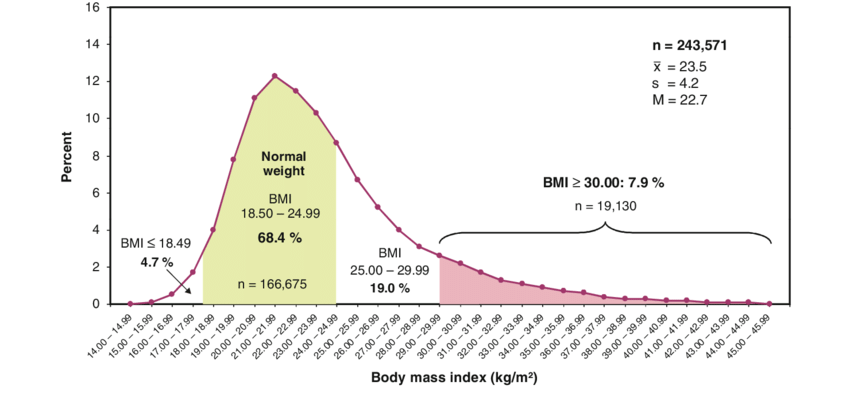
\epsfig{file=images/bmi_2,width=1.3\linewidth}}
%   ~\cite[]{aaron2023explain}
% \end{minipage}

\begin{figure}
  \centering
  % If you continue using \epsfig
  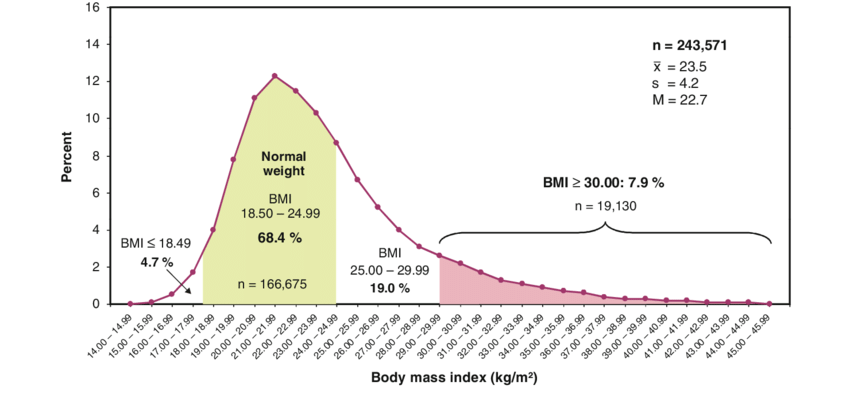
\epsfig{file=images/bmi_2,width=0.6\linewidth}
  % If you switch to \includegraphics from the graphicx package
  % 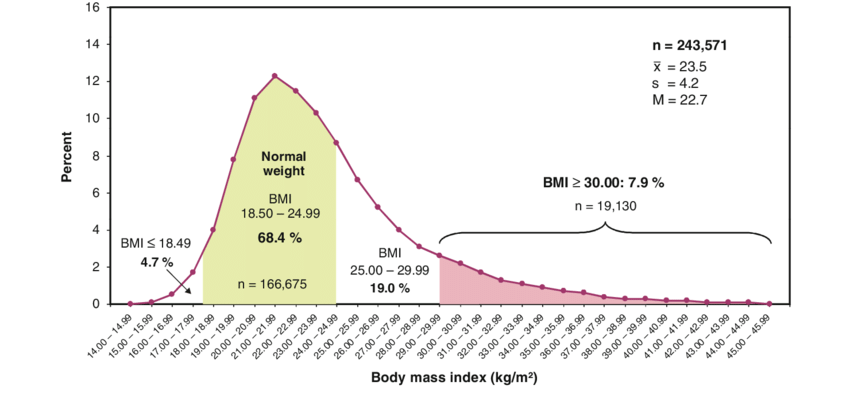
\includegraphics[width=0.6\linewidth]{images/bmi_2}
  \caption{BMI Categories~\cite{article}}
\end{figure}


% \begin{itemize}
% \pause
% \item  \textcolor{blue}{Likert scale}:  ``strongly disagree'', ``disagree'', ``agree'', or ``strongly agree'' in a survey.
% \pause
% \item \textcolor{blue}{Braun-Blanquet cover-abundance scale} is very common in vegetation analysis. 
% \end{itemize}

\end{frame}


%-----------------------------------------------------------------------------
\begin{frame}\frametitle{Clustering}

  Distance based clustering approach relies on the concept of similarity or distance between data points. The aim is to minimize the distance between data points within a cluster while maximizing the distance between data points in different clusters. Popular methods include K-means, hierarchical clustering, and DBSCAN, each using different metrics (e.g., Euclidean, Manhattan) to measure distance or similarity

  \begin{figure}
    \centering
    % If you continue using \epsfig
    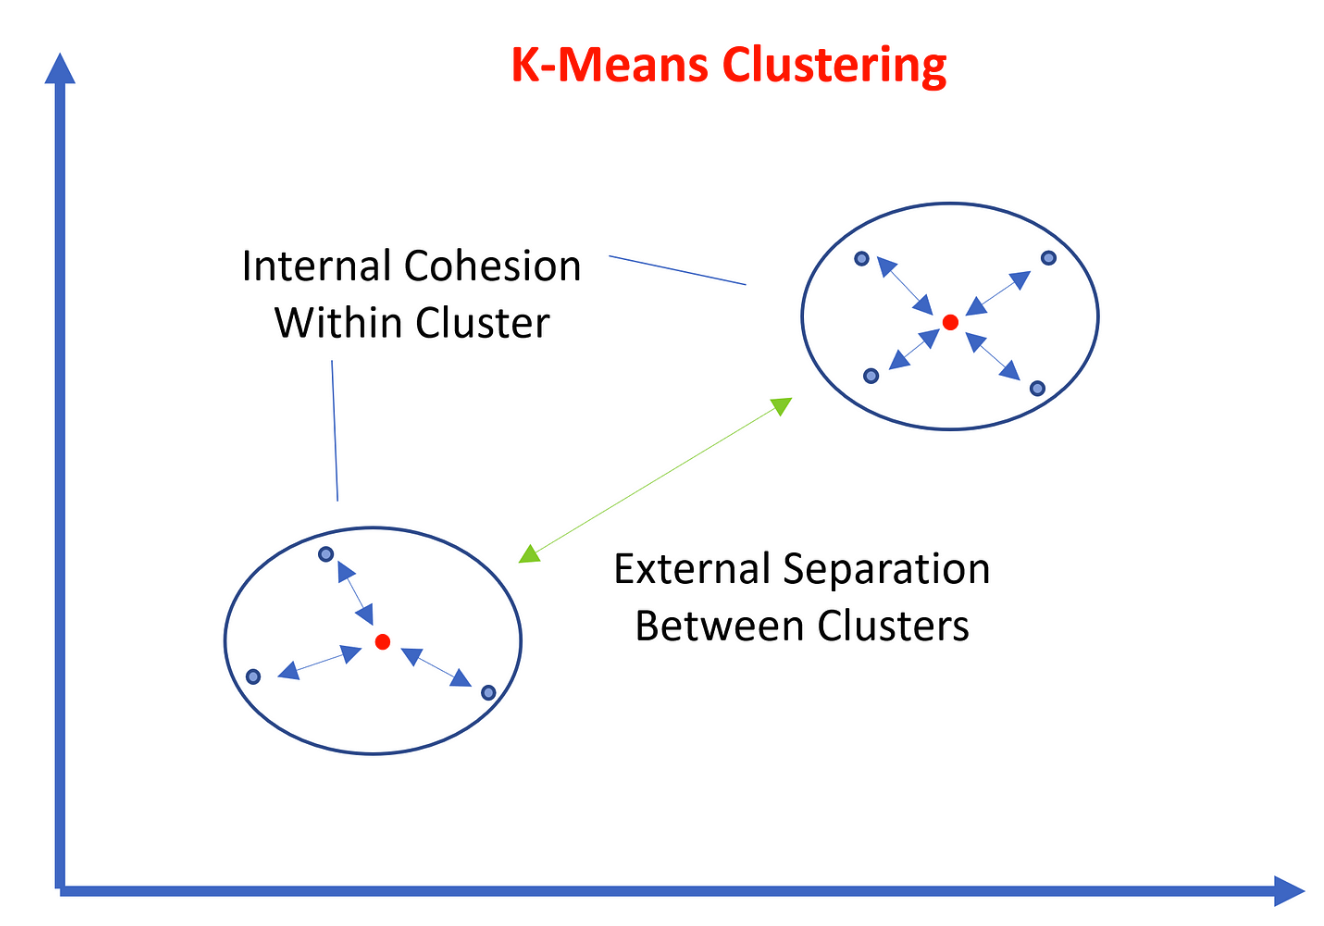
\epsfig{file=images/clustering_2,width=0.48\linewidth}
    % If you switch to \includegraphics from the graphicx package
    % 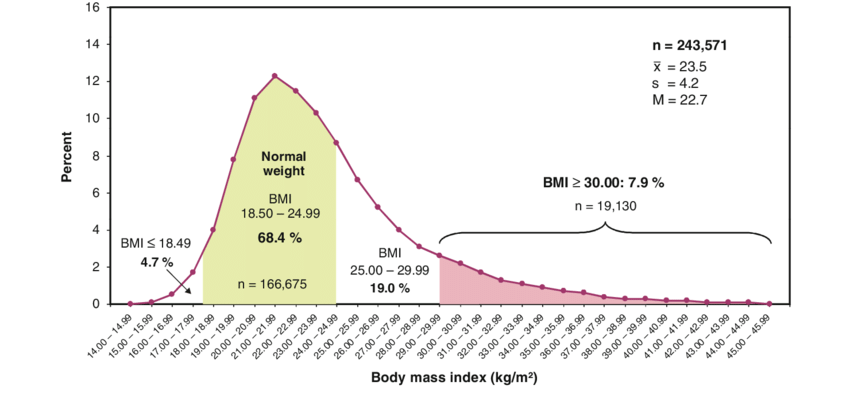
\includegraphics[width=0.6\linewidth]{images/bmi_2}
    \caption{Distance based Clustering~\cite{aaron2023explain}}
  \end{figure}

  % \begin{minipage}
  %   {0.5\textwidth}{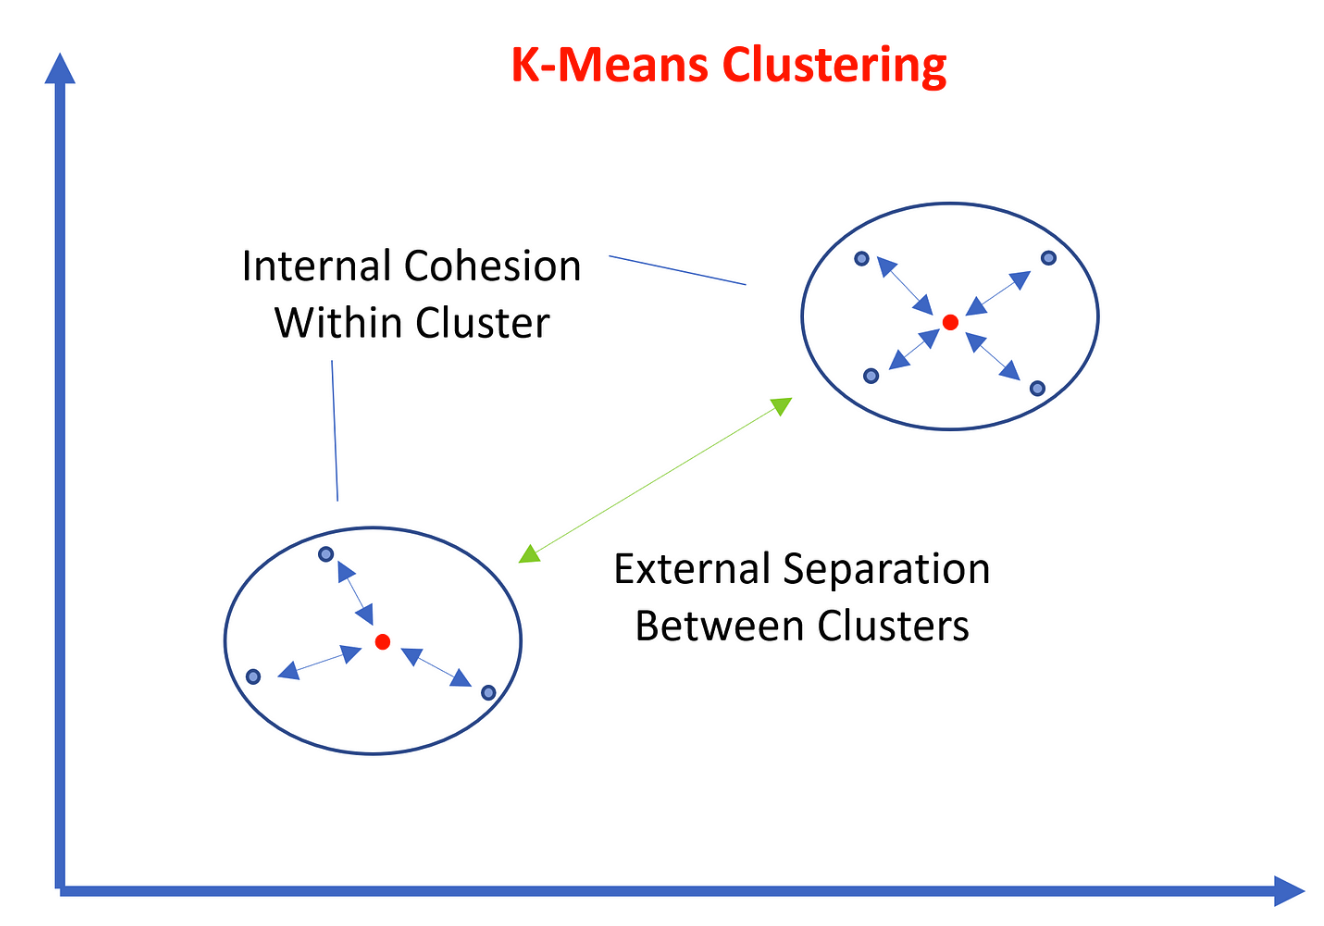
\epsfig{file=images/clustering_2,width=1.3\linewidth}}
  % \end{minipage}

% \begin{itemize}
%  \item 
% Data represented as a matrix $Y$ with dimensions $n\times m$ ($n$ could be species., $m$ could be sites) where
%   \begin{equation*} 
%       y_{ij} \in \{1,\ldots,q\} \hspace{25pt} i=1,\ldots,n \hspace{15pt} j=1,\ldots,m \hspace{15pt} q\;categories.
%   \end{equation*}
% \pause
%   \item \color{black}{For example, Spider data: }
%       \begin{itemize}
% 	\scriptsize
% 	\item $n=12$ species (rows)
% 	\item $m=28$ sites (columns).
% 	\item $q=4$ categories: Absence (0),\\ \hspace{2cm} Presences: (0,25\%] (1), (25,65\%] (2) and (65,100\%] (3)
% \pause
%       \end{itemize}
% \vspace*{-0.5in}
% \begin{minipage}{0.6\textwidth}{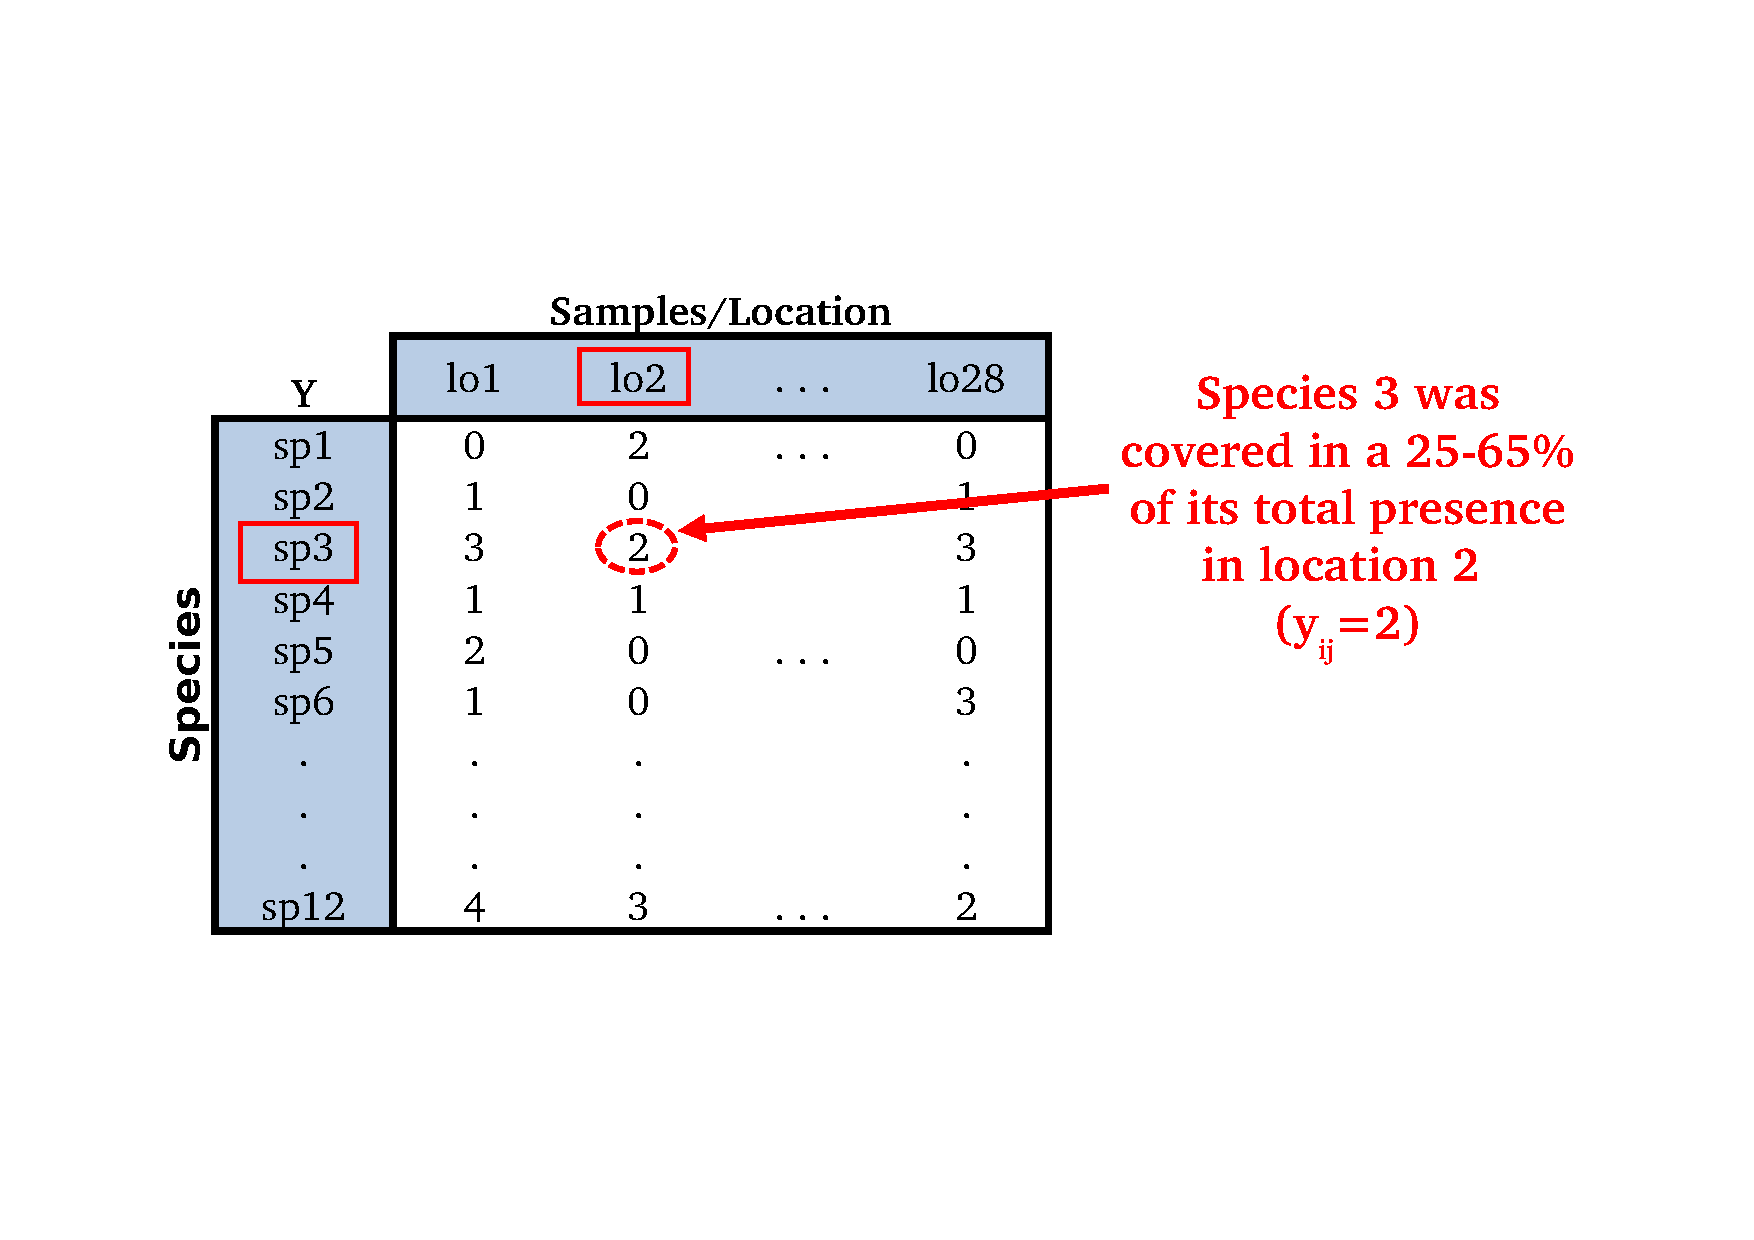
\epsfig{file=images/datamatrix_spider.pdf,width=1.3\linewidth}}\end{minipage}
% \end{itemize}

\end{frame}


%-----------------------------------------------------------------------------

\begin{frame}\frametitle{Finite Mixture Modeling}

  Unlike distance-based methods, statistical model-based clustering assumes that the data is generated from a mixture of finite distributions, where each component of the mixture represents a cluster. This approach tries to estimate the parameters of these distributions to optimize the fit between the model and the data.
  
  \begin{figure}
    \centering
    % If you continue using \epsfig
    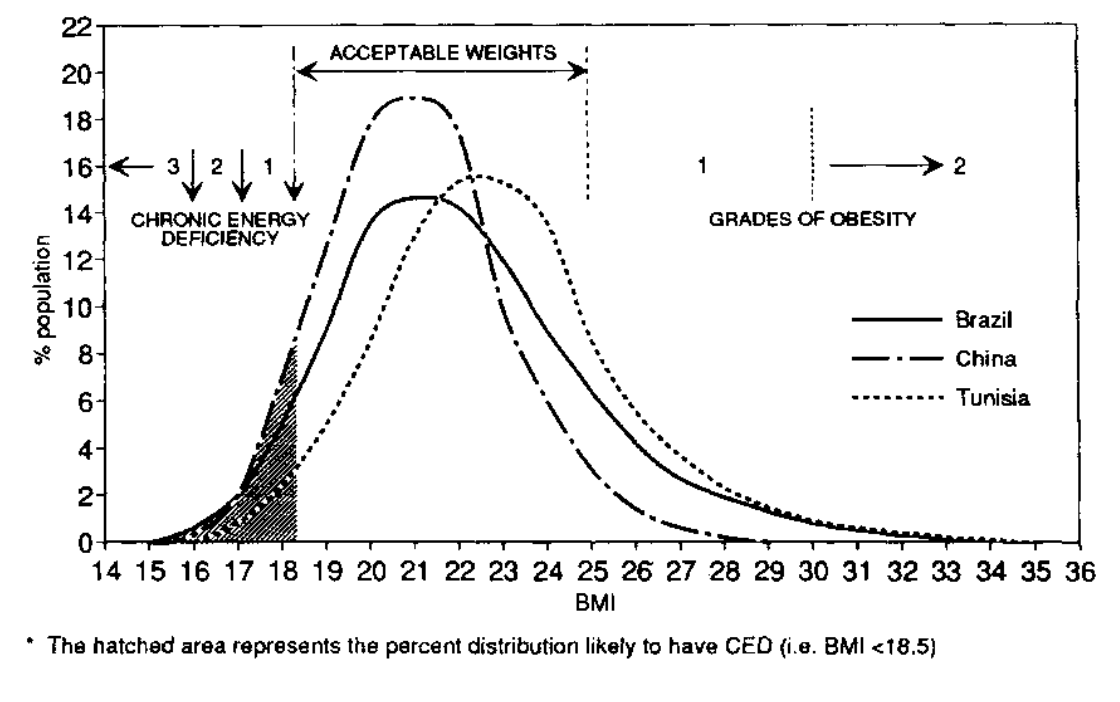
\epsfig{file=images/fmm_1,width=0.48\linewidth}
    % If you switch to \includegraphics from the graphicx package
    % 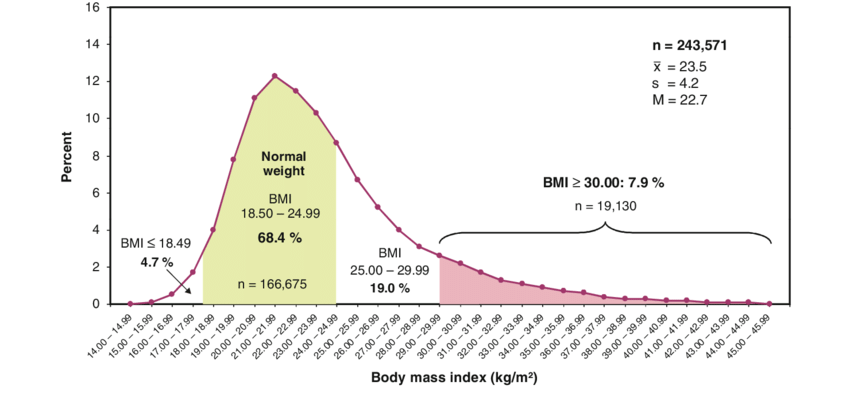
\includegraphics[width=0.6\linewidth]{images/bmi_2}
    \caption{mixture distribution between countries~\cite{shetty1994body}}
  \end{figure}
  
\end{frame}

%-----------------------------------------------------------------------------

\begin{frame}\frametitle{Bernoulli and Poisson distribution FMMS}

  \begin{figure}
    \centering
    \begin{minipage}{.48\linewidth}
      \centering
      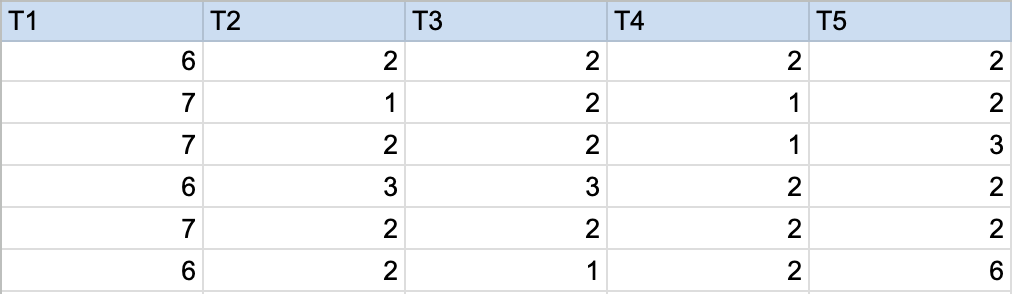
\epsfig{file=images/pmm,width=\linewidth}
      \caption{Apply Poisson  Distribution FMMs (for number of count)}
    \end{minipage}\hfill
    \begin{minipage}{.48\linewidth}
      \centering
      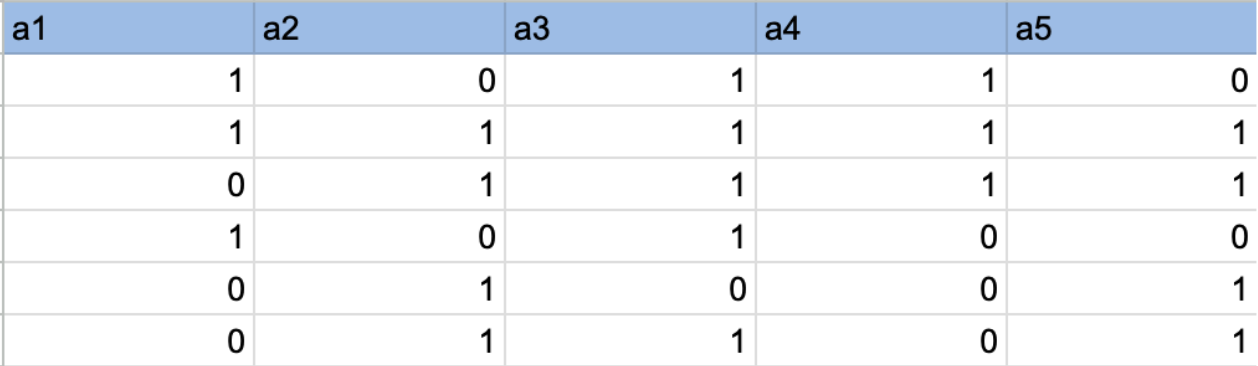
\epsfig{file=images/bmm,width=\linewidth}
      \caption{Apply Bernoulli Distribution FMMs}
    \end{minipage}
  \end{figure}
  
\end{frame}

% %--------------------------------------------------------
% \begin{frame}\frametitle{Background: Proportional odds model}

% Now, consider $Y$ has $c$ ordered categories.  For instance, let $c=3$ ( 1=''worse'', 2=''unchanged'', 3=''better'').

% \pause
% \begin{minipage}{0.5\textwidth}{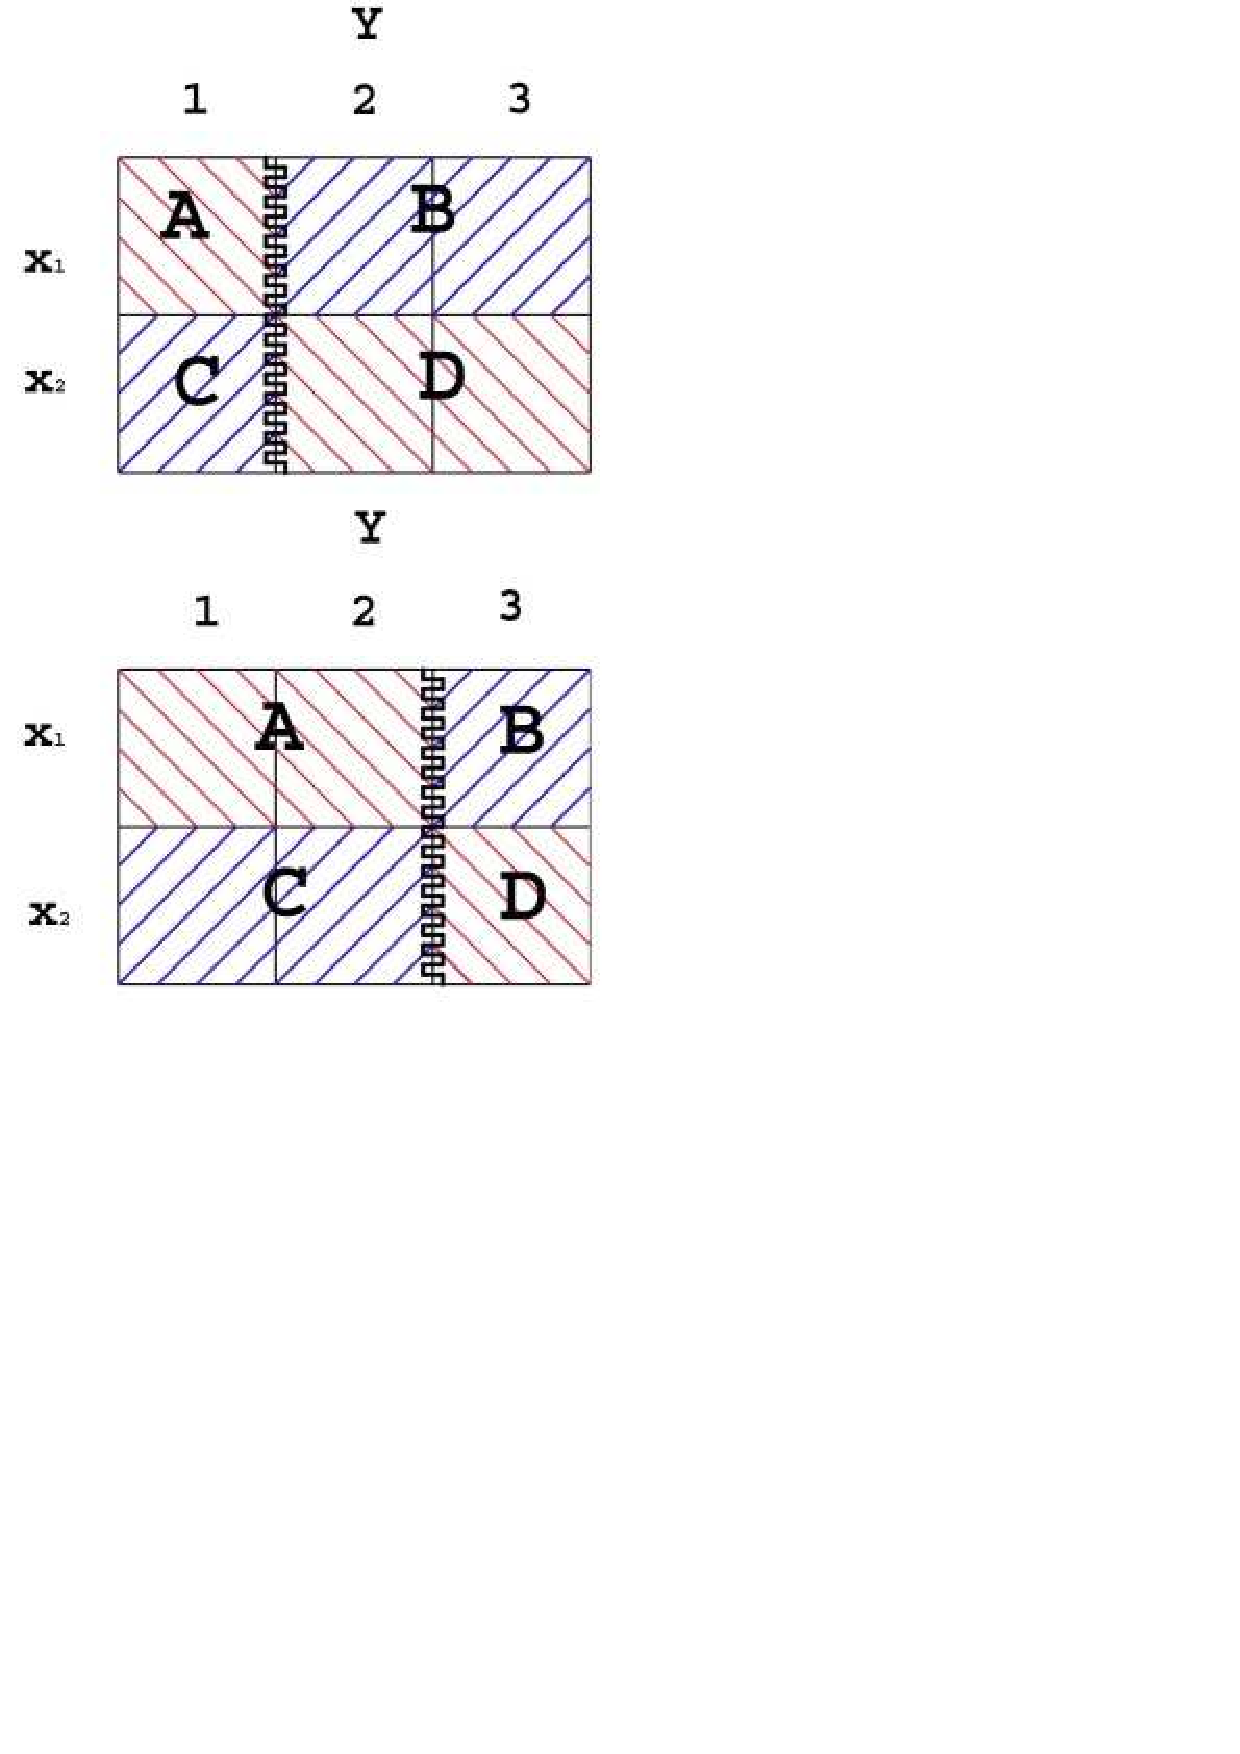
\epsfig{file=images/Pic2.pdf,width=1.3\linewidth}}\end{minipage}
% \begin{minipage}{0.45\textwidth}{\vspace{-1.5in}There are $c-1$  possible ways of collapsing a $c$-category response to a binary variable.\vspace{.2in}  \\  The proportional odds model implies that the odds
% ratios ($=\frac{A\times D}{B\times C}$) for describing effects of $X$ on the response variable are the same for each of these tables.
% }\end{minipage}
% \end{frame}

%--------------------------------------------------------
\begin{frame}\frametitle{Reference}
\bibliographystyle{plain}
\bibliography{reference}
\end{frame}

\end{document}
